\section{Concurrent programming}
Concurrency is an essential concept in computer science that enables multiple tasks to run simultaneously in a program.
This section introduces the concept of concurrent programming and discusses the different concepts associated with it.

\subsection{Sequential programming}
Before discussing concurrent programming, it is important to understand the concept of sequential programming.
Sequential programming is a programming paradigm in which one task is finished before the next one is started.
This can be seen as the default type of programming where one line of code is executed after another in a linear order.
Figure \ref{fig:concurrency_sequential} shows an example of a sequential program that executes a sequence of three tasks multiple times.

If there is no reason to execute tasks concurrently, then sequential programming is often the best choice as there is little to no overhead involved and it is easy to understand, debug and maintain.

\begin{figure}[H]
    \centering
    
\includegraphics[width=\textwidth]{figures/concurrency/sequential.pdf}
    \caption{Visualization of sequential programming.}
    \label{fig:concurrency_sequential}
\end{figure}


\subsection{Concurrent programming}
Concurrent programming is a programming paradigm in which multiple tasks are executed simultaneously.
There are many different ways to achieve concurrency but two main  categories are asynchronous programming and parallel programming.


\subsection{Asynchronous programming}
Asynchronous programming enables the concurrent execution of tasks without blocking others while processing one task at a time.
It is commonly used in systems involving I/O operations, such as network communication, where waiting for results can be time-consuming.
Rather than blocking the program, asynchronous programming allows for the execution of other tasks while waiting for an operation to complete.
This concept is illustrated in Figure \ref{fig:concurrency_concurrent}, where three tasks are executed multiple times asynchronously.

In asynchronous programming, coroutines are often utilized.
Coroutines are functions that can be paused and resumed, providing a flexible control flow.
Another common approach is to use callbacks, functions called upon task completion.

A fitting metaphor for asynchronous programming is a chef cooking, where he or she switches between preparing multiple dishes while waiting for others to cook.


\begin{figure}[H]
    \centering
    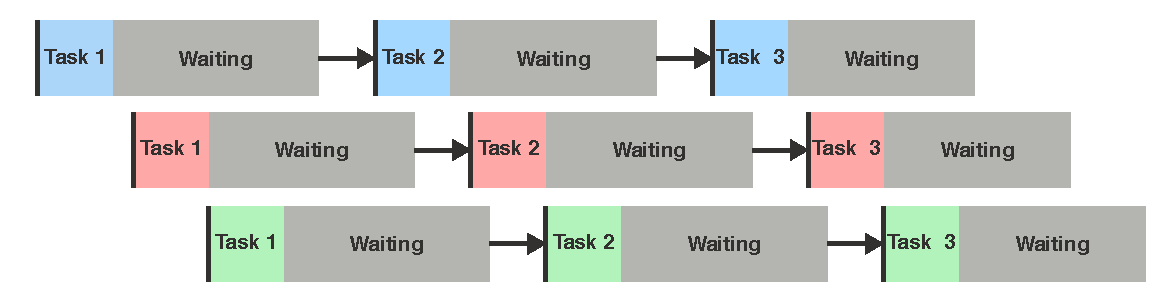
\includegraphics[width=\textwidth]{figures/concurrency/concurrent.pdf}
    \caption{Visualization of asynchronous programming.
        Each color represents work performed by a coroutine.}
    \label{fig:concurrency_concurrent}
\end{figure}


\subsection{Parallel programming}
Parallel programming, as opposed to asynchronous programming, enables the simultaneous processing of multiple tasks.
It offers substantial performance improvements, particularly for compute-intensive tasks, but requires a system with multiple processing units like a multi-core \gls{cpu} or a \gls{gpu}

Figure \ref{fig:concurrency_parallel} demonstrates an example of parallel programming, where multiple tasks are executed simultaneously.

Extending the chef metaphor, parallel programming is analogous to having multiple chefs collaboratively working in a kitchen.
This collective effort can greatly expedite the cooking process.
However, coordination and synchronization among the chefs are necessary to maintain order and prevent chaos.

\begin{figure}[H]
    \centering
    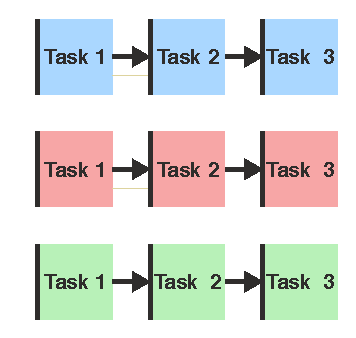
\includegraphics[width=.33\textwidth]{figures/concurrency/paralell.pdf}
    \caption{Parallel programming}
    \label{fig:concurrency_parallel}
\end{figure}


\subsection{Design patterns}
When designing a concurrent program, there are many factors to consider. The following questions can help guide the decision-making process:

\begin{itemize}
    \item Does task communication play a role in the program?
    \item Does the task necessitate significant memory usage?
    \item Can the task be executed in parallel?
    \item Is the task dependent on \gls{io} operations?
    \item Does the order of output matter for the program?
    \item Is minimizing latency crucial?
    \item Are there any potential bottlenecks in the program?
    \item Which tasks require substantial resource allocation?
\end{itemize}

Depending on the answers to these questions, different design patterns may be more suitable than others.
Figure \ref{fig:concurrency_concurrent_overlap} shows three different implementations of the same problem.

In the first implementation, each thread performs all tasks three tasks sequentially and independently.
The second implementation assigns each thread to a specific task, allowing them to repeatedly perform that task and pass the result to the next thread.
The third implementation is a combination of the two, where one thread is responsible for one task, while the other two receive data from the first thread and perform the remaining tasks.
This combined approach is particularly suitable when the first task involves \gls{io} operations.

\begin{figure}[H]
    \centering
    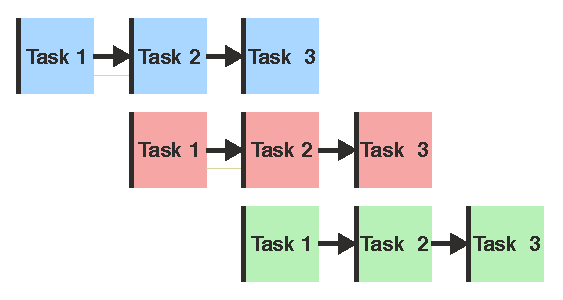
\includegraphics[width=.48\textwidth]{figures/concurrency/concurrent_overlap.pdf}
    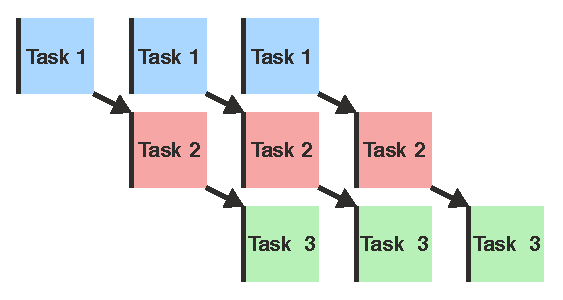
\includegraphics[width=.48\textwidth]{figures/concurrency/thread_per_task.pdf}
    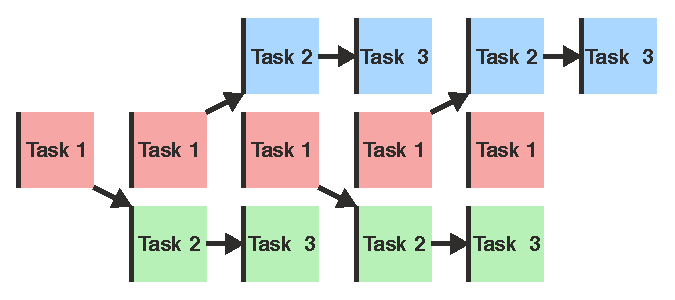
\includegraphics[width=.6\textwidth]{figures/concurrency/distribute.pdf}
    \caption{Three different implementations solving the same concurrent problem.}
    \label{fig:concurrency_concurrent_overlap}
\end{figure}


